\chapter{Manipulation of HBase}
%Intro\footnotemark\\
\par Lorem ipsum dolor sit amet, consectetur adipiscing elit. Aliquam facilisis massa quis orci volutpat, ut dictum tellus pulvinar. Nam vulputate diam a leo dignissim varius. Aenean nec tellus malesuada, tristique libero vitae, lacinia nibh. Donec quam libero, accumsan sollicitudin massa a, dictum gravida mauris.
\begin{spacing}{1.2}
%note en bas de page
\section{Creation of a BD }
\par Lorem ipsum dolor sit amet, consectetur adipiscing elit. Aliquam facilisis massa quis orci volutpat, ut dictum tellus pulvinar. Nam vulputate diam a leo dignissim varius. Aenean nec tellus malesuada, tristique libero vitae, lacinia nibh. Donec quam libero, accumsan sollicitudin massa a, dictum gravida mauris
\\
\begin{figure}[!htb] 
\begin{center} 
\includegraphics[width=1\linewidth]{Pictures/HBase/Manipulation of HBase/Creation of a BD/Creating a table and Verifying } 
\end{center} 
\caption{Creating a table and Verifying } 
\end{figure}  \FloatBarrier
\\

\par Lorem ipsum dolor sit amet, consectetur adipiscing elit. Aliquam facilisis massa quis orci volutpat, ut dictum tellus pulvinar. Nam vulputate diam a leo dignissim varius. Aenean nec tellus malesuada, tristique libero vitae, lacinia nibh. Donec quam libero, accumsan sollicitudin massa a, dictum gravida mauris
\\
\begin{figure}[!htb] 
\begin{center} 
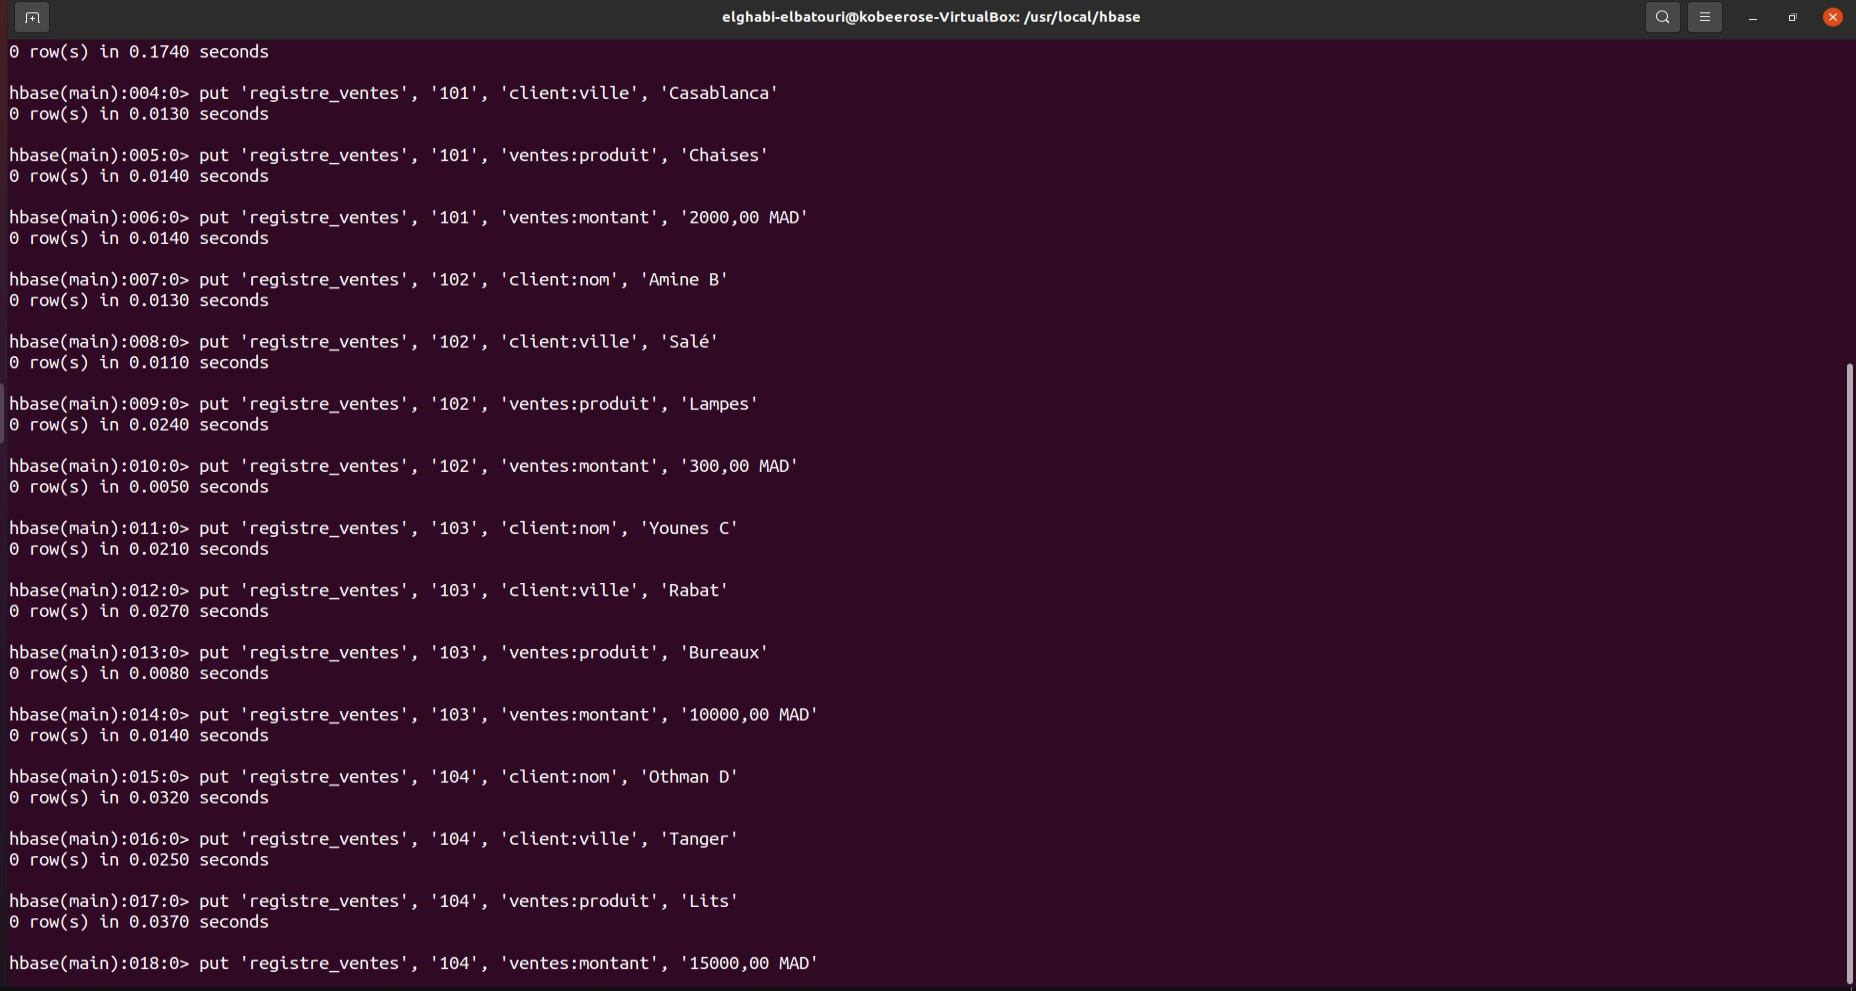
\includegraphics[width=1\linewidth]{Pictures/HBase/Manipulation of HBase/Creation of a BD/Inserting Values to the table} 
\end{center} 
\caption{Inserting Values to the table} 
\end{figure}  \FloatBarrier
\\

\par Lorem ipsum dolor sit amet, consectetur adipiscing elit. Aliquam facilisis massa quis orci volutpat, ut dictum tellus pulvinar. Nam vulputate diam a leo dignissim varius. Aenean nec tellus malesuada, tristique libero vitae, lacinia nibh. Donec quam libero, accumsan sollicitudin massa a, dictum gravida mauris
\\
\begin{figure}[!htb] 
\begin{center} 
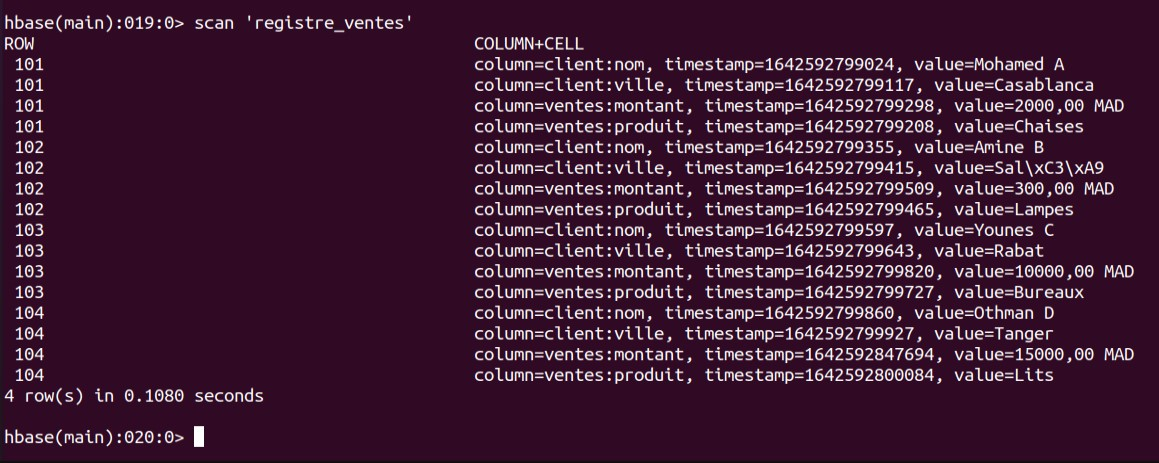
\includegraphics[width=1\linewidth]{Pictures/HBase/Manipulation of HBase/Creation of a BD/Checking the table} 
\end{center} 
\caption{Checking the table} 
\end{figure}  \FloatBarrier
\\

\par Lorem ipsum dolor sit amet, consectetur adipiscing elit. Aliquam facilisis massa quis orci volutpat, ut dictum tellus pulvinar. Nam vulputate diam a leo dignissim varius. Aenean nec tellus malesuada, tristique libero vitae, lacinia nibh. Donec quam libero, accumsan sollicitudin massa a, dictum gravida mauris
\\
\begin{figure}[!htb] 
\begin{center} 
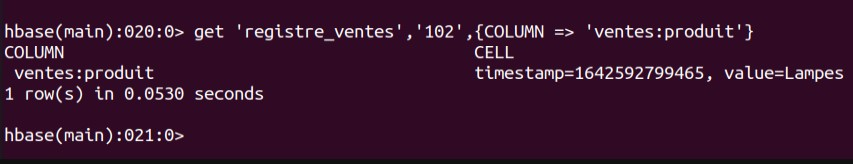
\includegraphics[width=1\linewidth]{Pictures/HBase/Manipulation of HBase/Creation of a BD/Display values of row 102} 
\end{center} 
\caption{Display values of row 102} 
\end{figure}  \FloatBarrier
\\

\end{spacing}